% ----- Consignes exo 8 ----- %
\begin{td-exo}[Problème de la coloration]\,\\ % 8 
	% add problem here
	\begin{enumerate}
		\item Montrer que \textsc{3-Coloration} est \(\mathcal{NP}\)-complet en effectuant une réduction à partir de \textsc{3-SAT}.

		Nous proposons la transformation polynomiale suivante à partir de \textsc{3-SAT}:

		Soit \(I\) une instance de \textsc{3-SAT} constitué d'un ensemble \(B = \left\{C_1, \ldots, C_m \right\}\) de clauses sur un ensemble \(X = \left\{x_1, \ldots, x_n \right\}\) de variables.
		Nous allons construire, à partir de la formule \(B\), un graphe \(G = (S, A)\) de manière que \(B\) soit satisfaisable si et seulement si \(G\) admet une coloration en 3 couleurs.

		\begin{itemize}
			\item Pour chaque variable \(x_i\), on pose \color{blue} \(T_i = (S_{i, 1}, A_{i, 1})\)\color{pagetext}~où \(S_{i, 1} = \{x_i, \ol{x_i}\}\) et \(A_{i, 1} = \{(x_i\ol{x_i})\}\), voir figure~\ref{fig:td1_ex08_2}.
			\item Pour chaque clause \(C_j\), on pose \color{red} \(V_j = (S_{j, 2}, A_{j, 2})\)\color{pagetext}~où \(S_{j, 2} = \{y_{j, 1}, y_{j, 2}, y_{j, 3}, y_{j, 4}, y_{j, 5}, y_{j, 6}\}\) et \(A_{j, 2} = \{(y_{j, 1}y_{j, 2}), (y_{j, 1}y_{j, 4}), (y_{j, 2}y_{j, 4}), (y_{j, 4}y_{j, 5}), (y_{j, 5}y_{j, 6}), (y_{j, 5}y_{j, 3}), (y_{j, 3}y_{j, 6})\}\), voir figure~\ref{fig:td1_ex08_3}.

			\item \(V_j\) est isomorphe à \(G_0 -\{u_0, u_1, u_2\}\). %add ref to fig here

			\item On pose \(T = (S_3, A_3)\) où \(S_3 = \{v_1, v_2\}\) et \(A_3 = \{(v_1v_2)\}\). %add ref to fig 3 here
			
			\item Pour chaque variable \(x_i\) on pose \(A_{i, 4} = \{v_2x_i, v_2\ol{x_i}\}\) et \(A_{i, 5} = \{(v_1y_{j, 6}, v_2y_{j, 6})\}\) pour tout \(j\in \{1, \ldots, m\}\).

			\item Enfin, \(A_{j, 6}\) est un ensemble de trois arêtes reliant, pour chaque clause \(C_j\), les trois sommets de type \(x_i\) ou \(\ol{x_i}\) correspondant aux littéraux de \(C_j\). Le premier littéral de \(C_j\) est relié à \(y_{j, 1}\), le deuxième à \(y_{j, 2}\) et le troisième à \(y_{j, 3}\), voir figure~\ref{fig:td1_ex08_4}.
		\end{itemize}
		Tous les graphes présentés ci-dessus sont donnés dans les figures ci-dessous:
		\begin{center}
			\begin{minipage}[b]{0.3\textwidth}
				\centering
				\ffigbox[\FBwidth]{%
\caption{\centering Graphe \(T_i\)}\label{fig:td1_ex08_2}
}{
    \fbox{
        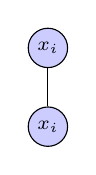
\begin{tikzpicture}[scale=1, main node/.style={circle, draw, fill=blue!20, inner sep=1pt, font=\scriptsize, minimum size=5mm, text=black}]
            % les sommets x_i
            \node[main node] (xi) at (-1,0) {\(x_i\)};
            \node[main node] (bxi) at (-1,-1) {\(\ol{x_i}\)};
            % on connecte les x_i aux bx_i
            \draw (xi) to (bxi);
        \end{tikzpicture}
    }
}
			\end{minipage}
			\hfill
			\begin{minipage}[b]{0.3\textwidth}
				\centering
				\ffigbox[\FBwidth]{%
\caption{\centering Graphe \(V_j\)}\label{fig:td1_ex08_3}
}{
    \fbox{
        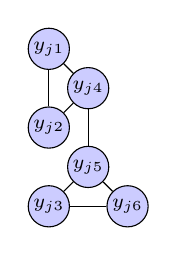
\begin{tikzpicture}[scale=1, main node/.style={circle, draw, fill=blue!20, inner sep=1pt, font=\scriptsize, minimum size=5mm, text=black}]
            % construction des triangles y_i
            \node[main node] (yj1) at (1, 0) {\(y_{j1}\)};
            \node[main node] (yj2) at (1, -1) {\(y_{j2}\)};
            \node[main node] (yj3) at (1, -2) {\(y_{j3}\)};
            \node[main node] (yj4) at (1.5, -0.5) {\(y_{j4}\)};
            \node[main node] (yj5) at (1.5, -1.5) {\(y_{j5}\)};
            \node[main node] (yj6) at (2, -2) {\(y_{j6}\)};
            
            % on connecte les y_i entre eux
            \draw (yj1) to (yj2);
            \draw (yj1) to (yj4);
            \draw (yj2) to (yj4);
            \draw (yj3) to (yj5);
            \draw (yj3) to (yj6);
            \draw (yj4) to (yj5);
            \draw (yj5) to (yj6);
        \end{tikzpicture}
    }
}
			\end{minipage}
			\hfill
			\begin{minipage}[b]{0.3\textwidth}
				\centering
				\ffigbox[\FBwidth]{%
\caption{\centering Graphe \(G_0\)}\label{fig:td1_ex08_4}
}{
    \fbox{
        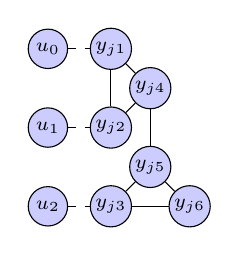
\begin{tikzpicture}[scale=1, main node/.style={circle, draw, fill=blue!20, inner sep=1pt, font=\scriptsize, minimum size=5mm, text=black}]
            % construction des triangles y_i
            \node[main node] (yj1) at (1, 0) {\(y_{j1}\)};
            \node[main node] (yj2) at (1, -1) {\(y_{j2}\)};
            \node[main node] (yj3) at (1, -2) {\(y_{j3}\)};
            \node[main node] (yj4) at (1.5, -0.5) {\(y_{j4}\)};
            \node[main node] (yj5) at (1.5, -1.5) {\(y_{j5}\)};
            \node[main node] (yj6) at (2, -2) {\(y_{j6}\)};

            \node[main node] (u0) at (0.2, 0) {\(u_0\)};
            \node[main node] (u1) at (0.2, -1) {\(u_1\)};
            \node[main node] (u2) at (0.2, -2) {\(u_2\)};
            
            % on connecte les y_i entre eux
            \draw (yj1) to (yj2);
            \draw (yj1) to (yj4);
            \draw (yj2) to (yj4);
            \draw (yj3) to (yj5);
            \draw (yj3) to (yj6);
            \draw (yj4) to (yj5);
            \draw (yj5) to (yj6);

            \draw[dashed] (u0) to (yj1);
            \draw[dashed] (u1) to (yj2);
            \draw[dashed] (u2) to (yj3);
        \end{tikzpicture}
    }
}
			\end{minipage}
		\end{center}

		Donner le nombre de sommets et le nombre d'arêtes de \(G\).
		Appliquer la construction sur l'instance \(X = \{x_1, x_2, x_3, x_4, x_5\}\) et \(B = \{C_1, C_2\}\) où \(C_1 = (x_1 \lor \ol{x_3} \lor \ol{x_4})\) et \(C_2 = (\ol{x_4} \lor x_2 \lor \ol{x_1})\).

		\item Montrer que le problème de \(4\)-coloration est \(\mathcal{NP}\)-complet en effectuant une réduction à partir de \textsc{3-Coloration}.

		\item Regarder la preuve pour des graphes planaires.
	\end{enumerate}
\end{td-exo}

% ----- Solutions exo 8 ----- %
\iftoggle{showsolutions}{ 
	\begin{td-sol}[]\ % 8
		On propose de visualiser le schéma de construction avec la figure~\ref{fig:td1_ex08_1} suivante:

		\ffigbox[\FBwidth]{%
\caption{\centering Construction de la réduction de \(3\)-\textsc{coloration} à partir de \(3\)-\textsc{sat}}\label{fig:td1_ex08_1}
}{
    \fbox{
        \begin{tikzpicture}[scale=1, main node/.style={circle, draw, fill=blue!20, inner sep=1pt, font=\scriptsize, minimum size=5mm, text=black}]
            % les sommets x_i
            \node[main node] (x1) at (-1,0) {\(x_1\)};
            \node[main node] (bx1) at (-1,-1) {\(\ol{x_1}\)};

            \node[main node] (x2) at (-1,-3) {\(x_2\)};
            \node[main node] (bx2) at (-1,-4) {\(\ol{x_2}\)};

            \node[main node] (x3) at (-1,-6) {\(x_3\)};
            \node[main node] (bx3) at (-1,-7) {\(\ol{x_3}\)};

            % construction des triangles y_i
            \node[main node] (y11) at (1, 0) {\(y_{11}\)};
            \node[main node] (y12) at (1, -1) {\(y_{12}\)};
            \node[main node] (y13) at (1, -2) {\(y_{13}\)};
            \node[main node] (y14) at (1.5, -0.5) {\(y_{14}\)};
            \node[main node] (y15) at (1.5, -1.5) {\(y_{15}\)};
            \node[main node] (y16) at (2, -2) {\(y_{16}\)};
            % et encore 2 triangles similaires pour les autres clauses en dessous des premiers
            \node[main node] (y21) at (1, -3) {\(y_{21}\)};
            \node[main node] (y22) at (1, -4) {\(y_{22}\)};
            \node[main node] (y23) at (1, -5) {\(y_{23}\)};
            \node[main node] (y24) at (1.5, -3.5) {\(y_{24}\)};
            \node[main node] (y25) at (1.5, -4.5) {\(y_{25}\)};
            \node[main node] (y26) at (2, -5) {\(y_{26}\)};

            \node[main node] (y31) at (1, -6) {\(y_{31}\)};
            \node[main node] (y32) at (1, -7) {\(y_{32}\)};
            \node[main node] (y33) at (1, -8) {\(y_{33}\)};
            \node[main node] (y34) at (1.5, -6.5) {\(y_{34}\)};
            \node[main node] (y35) at (1.5, -7.5) {\(y_{35}\)};
            \node[main node] (y36) at (2, -8) {\(y_{36}\)};
            % rajout des deux v_i
            \node[main node] (v1) at (3, 2) {\(v_1\)};
            \node[main node] (v2) at (4, 2) {\(v_2\)};
            

            % les aretes
            % on connecte les x_i aux bx_i
            \foreach \i in {1,2,3} {
                \draw (x\i) to (bx\i);
            }

            % on connecte les y_i entre eux
            \foreach \i in {1,2,3} {
                \draw (y\i1) to (y\i2);
                \draw (y\i1) to (y\i4);
                \draw (y\i2) to (y\i4);
                \draw (y\i3) to (y\i5);
                \draw (y\i3) to (y\i6);
                \draw (y\i4) to (y\i5);
                \draw (y\i5) to (y\i6);
            }

            % on connecte les v_i entre eux
            \draw (v1) to (v2);

            % left bus vertical pour collecter les xi
            \coordinate (lbt) at (-2,2);

            \foreach \i in {1,2,3} {
                \draw (x\i)  -- ($(x\i)+(-0.5,0.5)$)  -| (lbt);
                \draw (bx\i) -- ($(bx\i)+(-0.5,0.5)$) -| (lbt);
            }

            \draw (lbt) -- (v1);

            % right bus vertical pour collecter les y6
            \coordinate (rbt) at (3.5,0.5);

            \foreach \i in {1,2,3} {
                \draw
                    (y\i6) -- ($(y\i6)+(0.5,0.5)$) -| (rbt);
            }

            \draw (v1) -- (rbt);
            \draw (v2) -- (rbt);

            % draw small dashed line left of each y1, y2, y3 to indicate the clause literals
            \foreach \i in {1,2,3} {
                \draw[dashed] ($(y\i1)+(-0.8,0)$) -- (y\i1);
                \draw[dashed] ($(y\i2)+(-0.8,0)$) -- (y\i2);
                \draw[dashed] ($(y\i3)+(-0.8,0)$) -- (y\i3);
            }
        \end{tikzpicture}
    }
}


		En appliquant le schéma de construction à l'instance donnée, on obtient le graphe suivant:

		\ffigbox[\FBwidth]{%
\caption{\centering Application de la construction à l'instance donnée avec un exemple de coloration}\label{fig:td1_ex08_5}
}{
    \fbox{
        \begin{tikzpicture}[scale=1, main node/.style={circle, draw, fill=blue!20, inner sep=1pt, font=\scriptsize, minimum size=5mm, text=black}]
            % les sommets x_i
            \node[main node] (x1) at (-1,0) {\(x_1\)};
            \node[main node, fill=green!20] (bx1) at (-1,-0.8) {\(\ol{x_1}\)};

            \node[main node] (x2) at (-1,-1.8) {\(x_2\)};
            \node[main node, fill=green!20] (bx2) at (-1,-2.6) {\(\ol{x_2}\)};

            \node[main node] (x3) at (-1,-3.6) {\(x_3\)};
            \node[main node, fill=green!20] (bx3) at (-1,-4.4) {\(\ol{x_3}\)};

            \node[main node] (x4) at (-1,-5.4) {\(x_4\)};
            \node[main node, fill=green!20] (bx4) at (-1,-6.2) {\(\ol{x_4}\)};

            \node[main node] (x5) at (-1,-7.2) {\(x_5\)};
            \node[main node, fill=green!20] (bx5) at (-1,-8) {\(\ol{x_5}\)};
            

            % construction des triangles y_i
            \node[main node, fill=green!20] (y11) at (1, 0) {\(y_{11}\)};
            \node[main node] (y12) at (1, -1) {\(y_{12}\)};
            \node[main node, fill=red!20] (y13) at (1, -2) {\(y_{13}\)};
            \node[main node, fill=red!20] (y14) at (1.5, -0.5) {\(y_{14}\)};
            \node[main node, fill=green!20] (y15) at (1.5, -1.5) {\(y_{15}\)};
            \node[main node] (y16) at (2, -2) {\(y_{16}\)};
            % et encore 2 triangles similaires pour les autres clauses en dessous des premiers
            \node[main node] (y21) at (1, -3) {\(y_{21}\)};
            \node[main node, fill=green!20] (y22) at (1, -4) {\(y_{22}\)};
            \node[main node, fill=red!20] (y23) at (1, -5) {\(y_{23}\)};
            \node[main node, fill=red!20] (y24) at (1.5, -3.5) {\(y_{24}\)};
            \node[main node, fill=green!20] (y25) at (1.5, -4.5) {\(y_{25}\)};
            \node[main node] (y26) at (2, -5) {\(y_{26}\)};
            % rajout des deux v_i
            \node[main node, fill=red!20] (v1) at (3, 2) {\(v_1\)};
            \node[main node, fill=green!20] (v2) at (4, 2) {\(v_2\)};
            

            % les aretes
            % on connecte les x_i aux bx_i
            \foreach \i in {1,2,3,4,5} {
                \draw (x\i) to (bx\i);
            }

            % on connecte les y_i entre eux
            \foreach \i in {1,2} {
                \draw (y\i1) to (y\i2);
                \draw (y\i1) to (y\i4);
                \draw (y\i2) to (y\i4);
                \draw (y\i3) to (y\i5);
                \draw (y\i3) to (y\i6);
                \draw (y\i4) to (y\i5);
                \draw (y\i5) to (y\i6);
            }

            % on connecte les v_i entre eux
            \draw (v1) to (v2);

            % left bus vertical pour collecter les xi
            \coordinate (lbt) at (-2,2);

            \foreach \i in {1,2,3,4,5} {
                \draw (x\i)  -- ($(x\i)+(-0.5,0.5)$)  -| (lbt);
                \draw (bx\i) -- ($(bx\i)+(-0.5,0.5)$) -| (lbt);
            }

            \draw (lbt) -- (v1);

            % right bus vertical pour collecter les y6
            \coordinate (rbt) at (3.5,0.5);

            \foreach \i in {1,2} {
                \draw
                    (y\i6) -- ($(y\i6)+(0.5,0.5)$) -| (rbt);
            }

            \draw (v1) -- (rbt);
            \draw (v2) -- (rbt);

            % connect the y_i to the x_i according to the clauses
            \draw (x1) to (y11);
            \draw (bx3) to (y12);
            \draw (bx4) to (y13);

            \draw (bx4) to (y21);
            \draw (x2) to (y22);
            \draw (bx1) to (y23);
            
        \end{tikzpicture}
    }
}

		On peut aussi retirer les couleurs de ce graphe et essayer de les assigner manuellement.
		Les paires \((x_i, \ol{x_i})\) doivent être colorées avec des couleurs différentes, et \(v_1\) et \(v_2\) doivent être colorés avec des couleurs différentes. Les \(y_{j, 6}\) doivent être colorés différemment de \(v_1\) et \(v_2\).
		Avec ces seules contraintes, on peut trouver une coloration en 3 couleurs du graphe, ce qui correspond à une assignation de vérité pour les variables \(x_i\) qui satisfait les clauses \(C_j\) et on peut passer de l'une à l'autre de manière bijective.

		Les seules choses à considérer pour passer d'une coloration à une autre est la permutation des couleurs \(y_{j, 1}, y_{j, 2}\) et celles des \(x_i\) et \(\ol{x_i}\), l'extension de cette construction à des instances plus grandes est alors facile.

		\begin{enumerate}
			\item Il est facile de voir qu'avec la construction proposée on a bien une réduction de \textsc{3-SAT} vers \textsc{3-Coloration} et donc ce dernier est \(\mathcal{NP}\)-complet.
			\item Il suffit de considérer le graphe \(G'\) qui a les memes sommets et arêtes que \(G\) mais avec un sommet supplémentaire \(v\) connecté à tous les autres sommets de \(G\).
			Alors si \(G\) est 3-colorable, alors \(G'\) est 4-colorable (en coloriant \(v\) avec une nouvelle couleur).
			Inversement, si \(G'\) est 4-colorable, alors \(v\) doit être colorié avec une couleur différente de celle de tous les autres sommets de \(G\), ce qui implique que \(G\) est 3-colorable.
		\end{enumerate}
	\end{td-sol}
}{}
